
\documentclass[a4paper,12pt]{article}
\usepackage[utf8]{inputenc}
\usepackage[T1]{fontenc}
\usepackage{graphicx}
\title{Esercizi su UDP (pagine 37–38)}
\author{}
\date{}

\begin{document}
\maketitle

\section*{Esercizi su UDP}

\begin{enumerate}
  \item[7)] \textbf{Compilare ed eseguire il secondo esempio.}\\
    \emph{Risposta:}\\
    \begin{figure}[h]
      \centering
      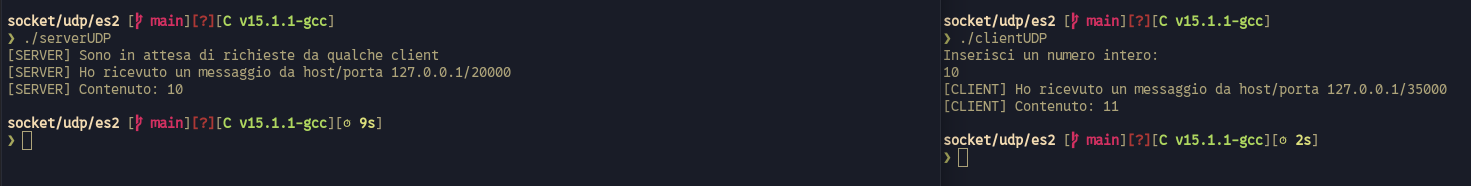
\includegraphics[width=0.8\linewidth]{esecuzione.png}
      \caption{Output dell'esecuzione del secondo esempio}
    \end{figure}

  \item[8)] \textbf{Modificare il secondo esempio per costruire una semplice sommatrice.}\\
    \emph{Answer:}\\
    \begin{figure}[h]
      \centering
      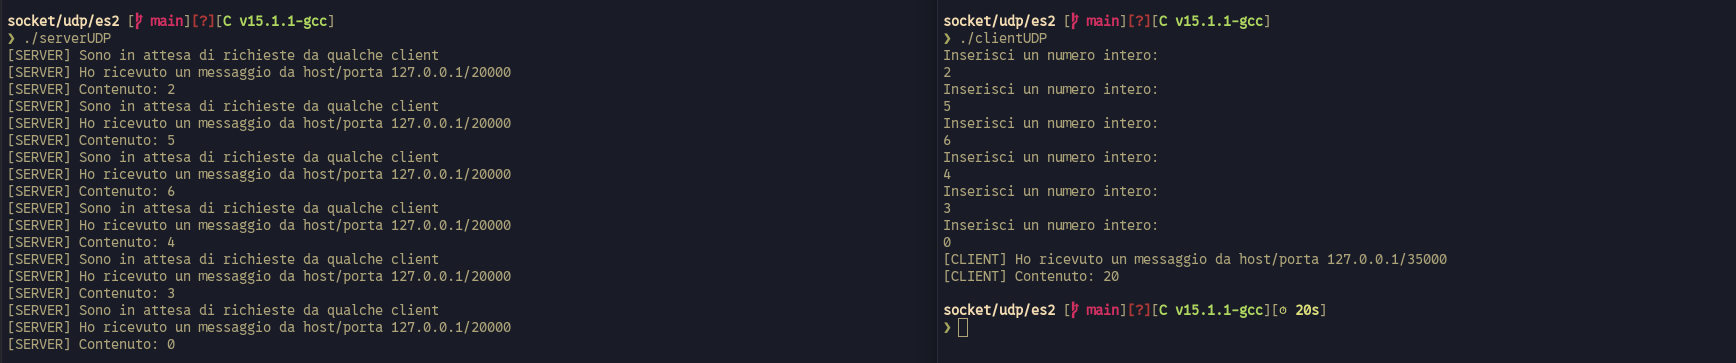
\includegraphics[width=0.8\linewidth]{sommatrice.png}
      \caption{Funzionamento della sommatrice UDP}
    \end{figure}
\end{enumerate}

\section*{Esercizio 9: sommatrice UDP e perdita di pacchetti}

Usare la sommatrice su due macchine distinte provando, sulla macchina del client, a staccare il cavo di rete prima di un invio di un dato, ad esempio:
\begin{itemize}
  \item Digitare “2345” + INVIO
  \item Digitare “5187” + INVIO
  \item Staccare il cavo
  \item Digitare “2” + INVIO
  \item Riattaccare il cavo e aspettare 30\,s che il sistema operativo si riassesti
  \item Digitare “1” + INVIO
  \item Digitare “0” + INVIO
\end{itemize}
\textbf{Domande:} Che somma leggo? È corretta?\\
\emph{Risposta:}\\
Il server somma solo i pacchetti effettivamente arrivati: 
\[2345 + 5187 + 1 + 0 = 7533\]
(l'elemento “2” è andato perso durante la caduta del collegamento). 
Il risultato corretto sarebbe stato 
\[2345 + 5187 + 2 + 1 + 0 = 7535.\]
Se anche la risposta “7533” andasse persa, il client resterebbe bloccato in ricezione. 
Per garantire affidabilità su UDP è necessario implementare un protocollo applicativo con ACK, timeout e ritrasmissione (oppure utilizzare TCP).
\end{document}
